\documentclass[12pt,a4paper]{report}
\usepackage{amsmath}%Class to implement all the mathematics symbols and equations in the file
\usepackage{caption}
\usepackage[pdftex]{graphicx}
\usepackage{url}
\usepackage[bookmarks, colorlinks=false, pdfborder={0 0 0}, pdftitle={Design Report}, pdfauthor={<Name of the author>}, pdfsubject={Design Report IITKMS}, pdfkeywords={IITKMS,IIT}]{hyperref} % help create hyperlink to different content

%% To edit your report, modify different .tex file in the folder you are in
\begin{document}
\renewcommand\bibname{References} 
% Add a title page to your document by editing title.tex file
\begin{titlepage}
	
	\begin{center}
		
		\Large \textbf {IITK Motorsports Formula Bharat 2017 Design Report}\\[0.5in]
		
		%       \small \emph{Submitted in partial fulfillment of\\
		%        the requirements for the award of the degree of}
		\vspace{3in}
		
\includegraphics[width=0.25\textwidth]{fig/iitkmslogo}\\[0.1in]
%		{ IITK Motorsports }\\[0.5in]
		
		% Submitted by
		\normalsize  by\\ Name of people involved
		
		
		\vfill
		
		%% Bottom of the page
		
\includegraphics[width=0.25\textwidth]{fig/iitklogo}\\[0.1in]
		
		%\normalsize
		\textsc{IITK Motorsports}\\
		\textsc{Indian Institute of Technology, Kanpur}
		
		
	\end{center}
	
\end{titlepage}

\pagenumbering{roman} % This keeps the page numbering in roman numerals before you actually start the report
\tableofcontents
\listoftables
\listoffigures
\newpage
\pagenumbering{arabic}% This keeps the page numbering in arabic numerals when you actually start the report

% Modify the respective file in order to edit your report
\chapter{Brake Rotor}
\section{Introduction}
Intro
\section{Material selection for the rotor}


Since the results of the analysis were satisfactory with an average factor of safety of around 5 and a mass of (mass), we decided to finalize this model for our rear rotor.

\begin{center}
	\begin{tabular}{lll}
		1 & 2 & 3 
	\end{tabular}
	\captionof{table}{Tablename}
\end{center}
	

\chapter{Pedal Assembly}

\section{Introduction}
The brake pedal applies an input force from driver's foot to the braking system. Design and construction of this part greatly effects how a brake system operates and how the driver feels.Long pedals reduce the pedal force required to stop a vehicle. However, long pedals have long travel. They can feel spongy to the driver. The b
\begin{enumerate}
\item[1.] High machinability
\item[2.] High strength
\item[3.] Good weldability
\item[4.] Low cost because of easy manufacturability
\item[5.] Yield strength($3.51*10^2 \ N/m^2$) is also higher than aluminum
\end{enumerate}

\chapter{Balance bar}

\section{Introduction}
Generally cars have 60\% braking force front biased and 40\% rear biased, this is because the dynamic weight transfer is in front while braking.\\
In lay man's terms, front weight increases during brake, thus requiring more energy to stop. Hence balanced bar is used.\\
\section{Designing}
\section{First Iteration}
We designed our own balance bar because this allows us to make it according to the dimensions we need. It also reduces the cost as manufacturing a balance bar is relatively cheaper than buying one.\\
The balance bar was made according to the dimensions derived from the available bearing and female rod ends. Stress analysis was carried out on solidworks to see if it can bear the force on it during braking.
\begin{figure}[htb]
	\centering
	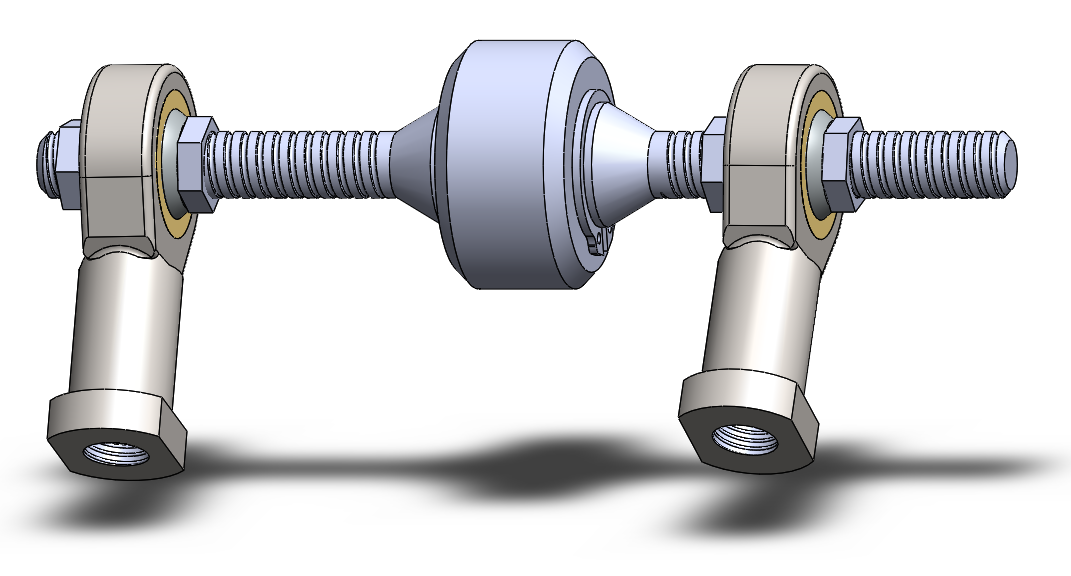
\includegraphics[scale=0.35]{fig/bb}
	\caption{Balance Bar}
	\label{fig:label}
\end{figure}


\chapter{Brake Assembly}

\section{Master Cylinder Mount}
The master cylinder mount has to be designed very carefully as it experiences a very large force perpendicular to itself and therefore has a very large tendency to bend.\\
\textbf{Material Selection}\\
As the main point for material selection is strength of the mount and weight, aluminum of thickness 4mm is used.\\
\textbf{Design}\\
The master cylinder mount has to be designed such that it can withstand large forces. Therefore, we have attached plates perpendicular to the main mount and appropriate analysis has been carried out on CAD models. It was designed to give a brake bias ratio along with the balance bar in order to keep the pushrods straight.

\chapter{Calculations}

\section{Introduction}
The calculations of various parameters are at the core of the braking system design and are necessary for us to select the specific models of the components of the braking system. Adding to that, they were needed to decide the dimensions of the components we designed and manufactured. Furthermore, they gave us a clear estimate of our vehicle's performance in the tests and events.
To begin with the calculations regarding the braking system they had to be categorized as :-
\textbf{Dynamics Of Braking}\\
It covers the behavior of the vehicle during braking and the behavior during peak deceleration was considered.
\textbf{Brake fluid volume calculations}\\
This part comes into picture due to need of brake fluid volume requirements for various components have to be met in order to assure that the brake pads make good contact with the brake rotors and apply the large enough force we desire.


\phantomsection
\addcontentsline{toc}{chapter}{References}
\begin{thebibliography}{99}
	%% provide a citation name below, it helps in setting up references when using in the text
	\bibitem{citation-1-name-here}Roy Featherstone. Rigid Body Dynamics Algorithms.  Springer, New York, 2008, \url{https://www.springer.com/it/book/9780387743141}
	\bibitem{silviothesis}Silvio Traversaro. Modelling, Estimation and Identification of Humanoid Robots Dynamics, \url{https://traversaro.github.io/preprints/traversaro-phd-thesis.pdf}
	
\end{thebibliography}

\end{document}
